\documentclass[11pt]{article}
\usepackage{tocloft}
\usepackage{graphicx}
\usepackage{calc}
\usepackage{amssymb}
\usepackage{color}
\usepackage{array}
\usepackage[sc]{mathpazo}
\usepackage{url}
\usepackage[final]{pdfpages}
\usepackage{amsmath}

%\linespread{1.05}
\oddsidemargin=0pt
\evensidemargin=0pt
\textwidth=6.5in
\topmargin=0pt
\headheight=0pt
\headsep=0pt
\textheight=9in
% EXPERIMENTAL
%\parindent=0pt
%\parskip=3pt
\setlength{\parindent}{0cm}
\newcommand\secfont{\fontfamily{cmss}\selectfont}%\textwidth 5.5truein
\newcommand\pifheading[1]{{\secfont\textbf{#1}:}}
%\oddsidemargin -0.40truein
%\textheight 8.0truein
%\topmargin -0.25truein
\def\lo{
\mathrel{\raise.3ex\hbox{$<$}\mkern-14mu\lower0.6ex\hbox{$\sim$}}
}
\def\hi{
\mathrel{\raise.3ex\hbox{$>$}\mkern-14mu\lower0.6ex\hbox{$\sim$}}
}

\textwidth = 6.6 in
\textheight = 9.1 in
\oddsidemargin = -0.05 in
\evensidemargin = +0.05 in
\topmargin = -.1 in
\headheight = 0.0 in
\headsep = 0.0 in
\parskip = 0.06in
\newcommand\registered{{\ooalign{\hfil\raise .00ex\hbox{\scriptsize R}\hfil\crcr\mathhexbox20D}}}

%% Define a new 'leo' style for the package that will use a smaller font.
\makeatletter
\def\url@leostyle{%
  \@ifundefined{selectfont}{\def\UrlFont{\sf}}{\def\UrlFont{\small\ttfamily}}}
\makeatother
%% Now actually use the newly defined style.
\urlstyle{leostyle}

%\pagestyle{empty}
%\includeonly{previous,proposal_references}
%\includeonly{proposal_references}
%\includeonly{previous}

% TOC

\begin{document}
%%%%%%%%%%%%%%%%%%%%%%%%%%%%%%%%%%%%%%%%%%%%%%%%%%%%%%%%%%%%%%%%%%%%%
\begin{center}
\textbf{\Large
AST101: Our Corner of the Universe \\
\vspace*{0.1cm}
Lab 4: Parallax Prelab
}
\end{center}

\vspace*{0.5cm}

{\Large Name:}\vspace*{0.5cm}\\\hrule
{\Large Student number (SUID):}\vspace*{0.5cm}\\\hrule
{\Large Lab section:}\vspace*{0.5cm}\\\hrule
{\Large Group Members:}\vspace*{0.5cm}\\\hrule
\vspace*{0.5cm}

%%%%%%%%%%%%%%%%%%%%%%%%%%%%%%%%%%%%%%%%%%%%%%%%%%%%%%%%%%%%%%%%%%%%%
\section{Introduction}

Recall that one of the issues that lead to the development of the celestial sphere model was the notion that stars do not exhibit parallax; that is, to the naked eye, the position of stars relative to one another never appear to alter in even the slightest. If the stars are not all the same distance away, then they ought to at times appear closer together or farther apart. This lab will explore the concept of parallax, and culminate with the realization that even though the stars ARE different distances away, we never could've found this with the tools available at the time. 

\subsection*{Materials}

You will need a friend; one of you needs a smartphone or digital camera. You'll also need the SU Quad or another open space outdoors.

\subsection*{Objective}

To prepare yourself to measure the effect of parallax on what we observe.

\newpage

\section{Outdoor Demo}

\begin{center}
	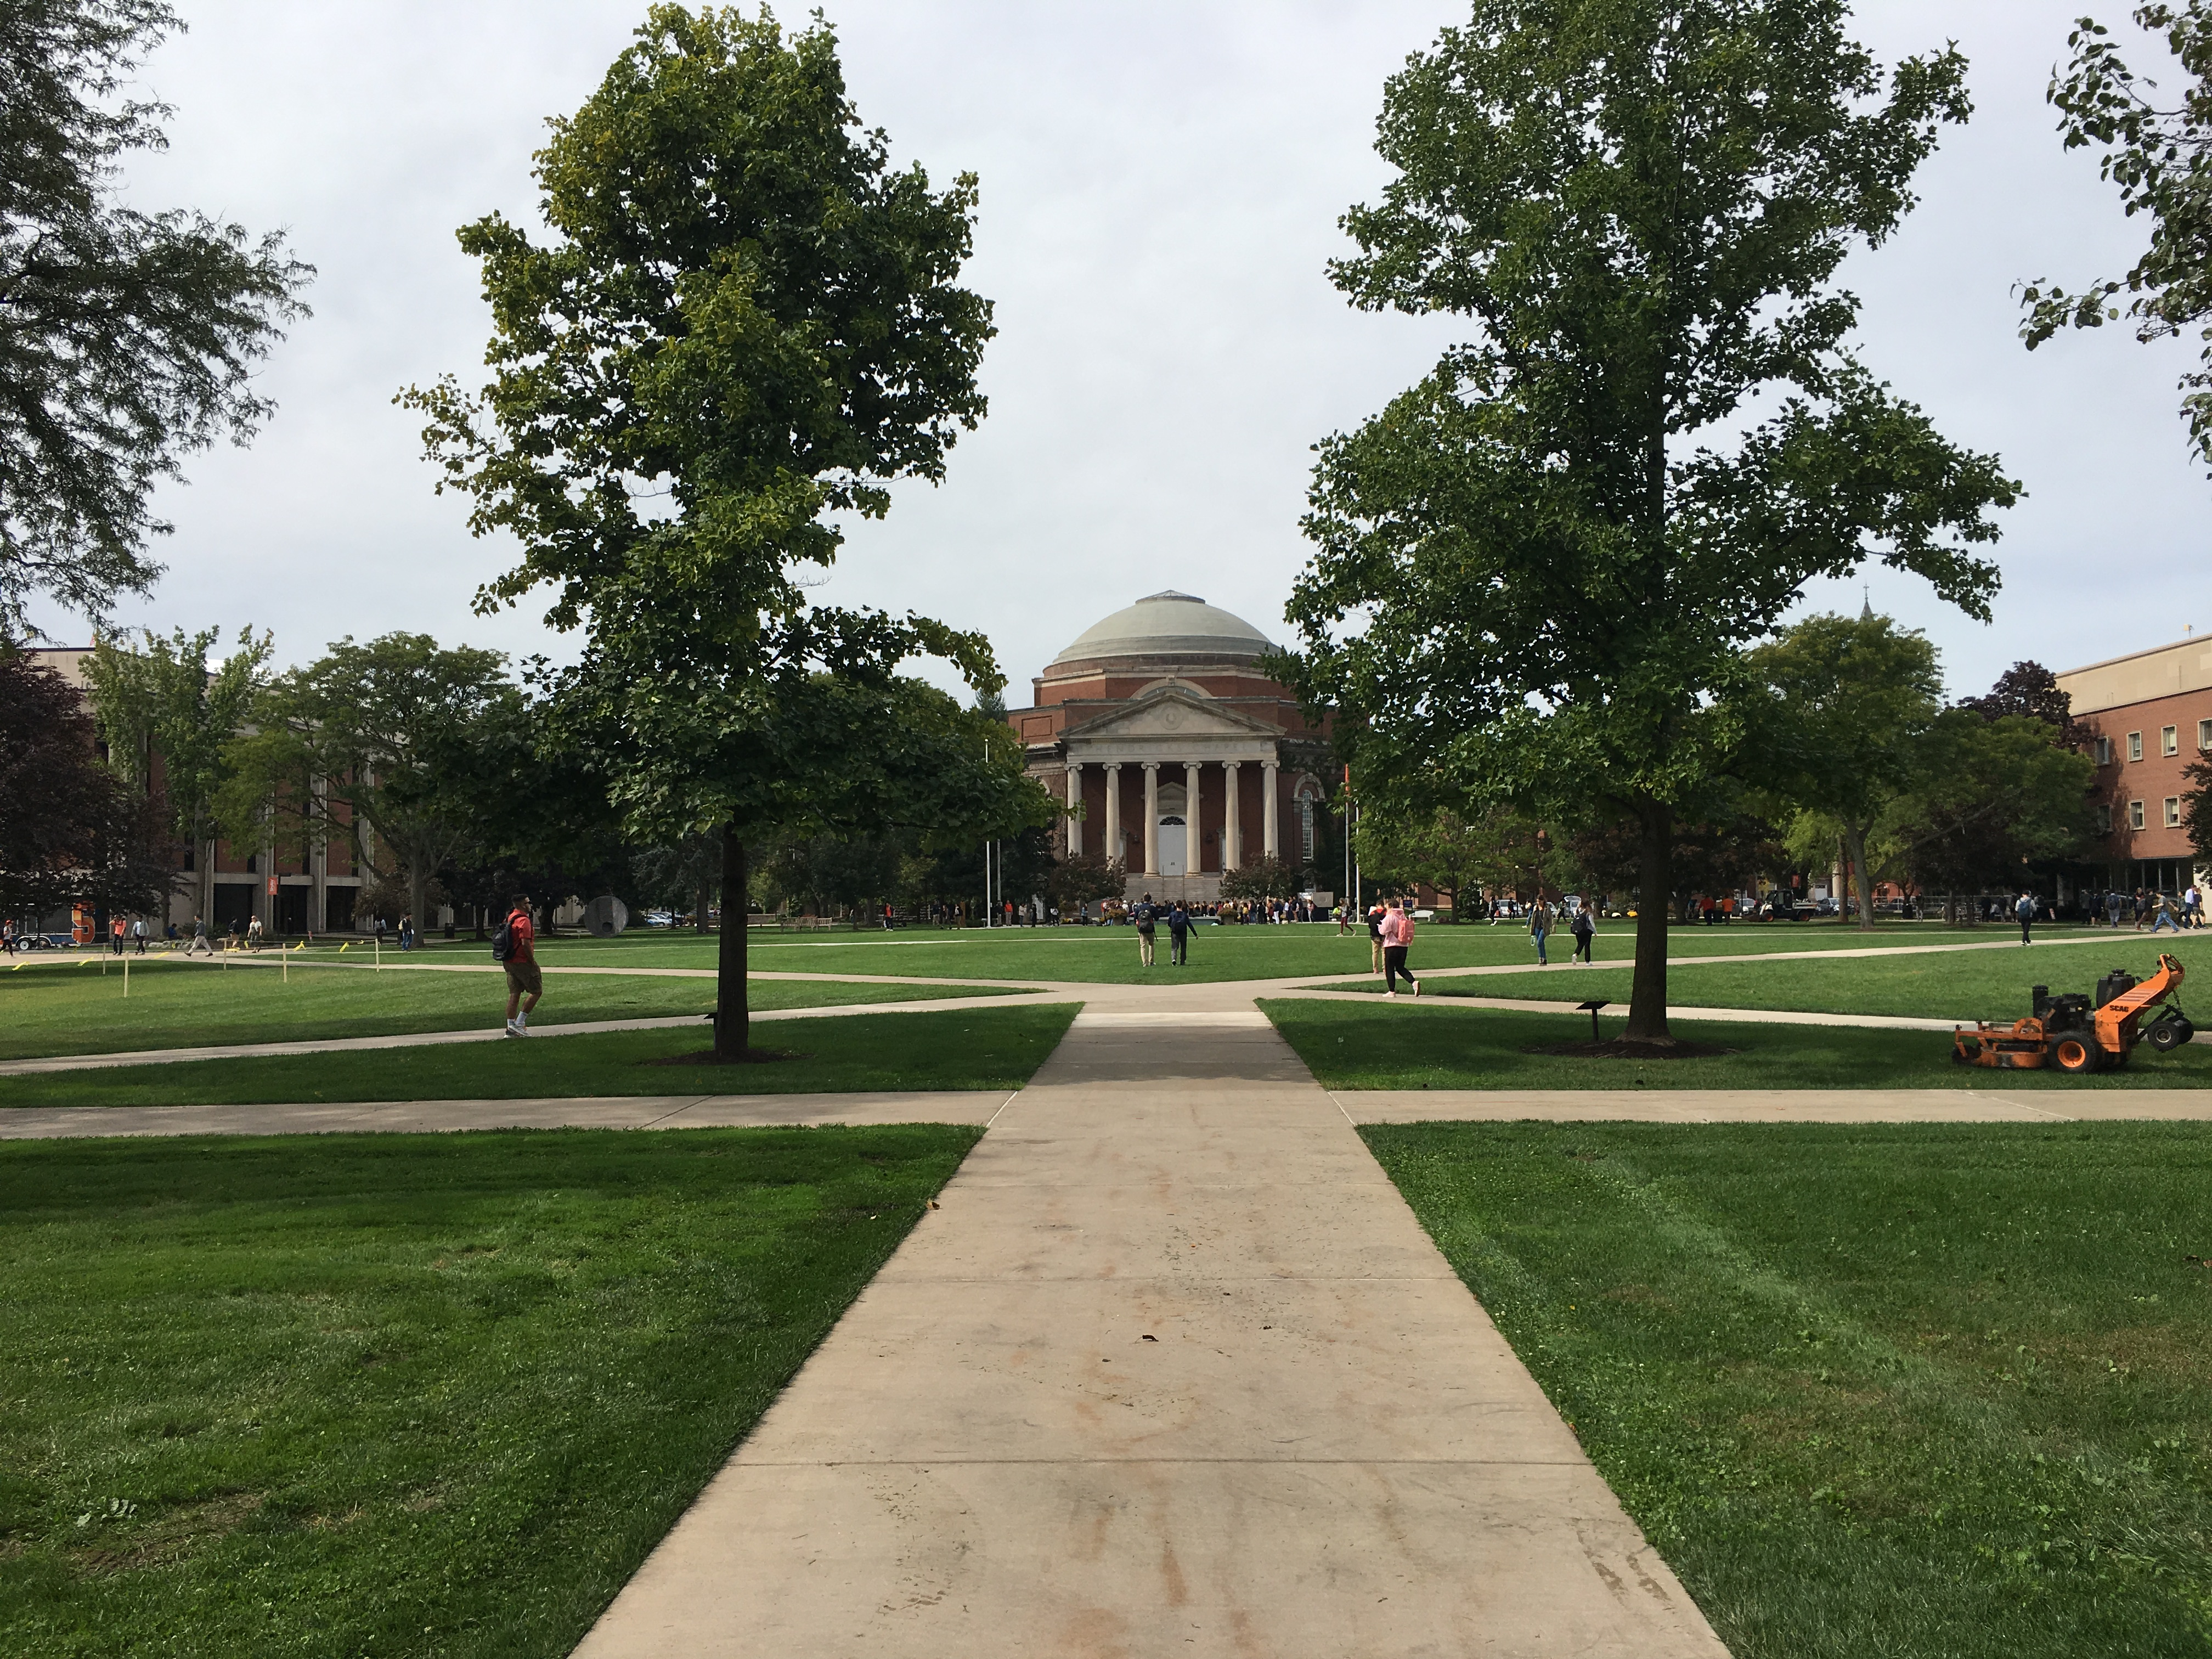
\includegraphics[width=150mm, scale=0.5]{Hall_of_Engineering}
\end{center}
Stand in front of the Hall of Engineering on the quad, and face Hendricks Chapel. Your view should be the same as the picture above. You can also use any other large open space outdoors.\\ 

\textbf{Question 1.} Hold your index finger directly in front of your nose, and close your left eye while keeping your right eye open. As you look at your index finger, does it appear to be in line with Hendricks, to the left of Hendricks, or to the right of Hendricks?\\

\vspace*{1.5cm}
\hrulefill

\newpage

\textbf{Question 2.} Now close your right eye and keep your left eye open. Does your index finger appear to be in line with Hendricks, to the left of Hendricks, or to the right of Hendricks?\\

\vspace*{1.5cm}
\hrulefill\\

\textbf{Question 3.} Why does your finger appear to change sides?\\

\vspace*{1.5cm}
\hrulefill\\
This is the notion of \textbf{parallax}! \\

\textbf{Question 4.} Now, hold your index finger farther away from your face, and repeat the exercise, observing your finger with just your left and just your right eye. Does your index finger still appear to move? Does it still move by the same amount?\\

\vspace*{1.5cm}
\hrulefill\\

\textbf{Question 5.} Do objects that are closer or farther away exhibit more or less parallax?\\

\vspace*{1.5cm}
\hrulefill

\newpage

You'll need a smartphone or digital camera for this. If you don't have one, work together with a classmate in your lab who does. 

Have a friend stand a few meters in front of you. The objective here is to use parallax to think about how far away from you they are. (You and a friend can use the same pictures to do the prelab, where one of you is the ``model'', the other operates the camera, and both of you think about the answers. You will each need your own copy of this prelab, though.)

Take a picture of them with your camera. Then move your camera a little bit to the side, and take another picture. The analogy is:

\begin{itemize}
	\item Your two camera positions are two different observing positions (on Earth)
	\item Your friend is a nearby object (planet, star) that you are trying to determine the distance to
	\item Hendricks Chapel is the background of stars that are far away
	\end{itemize}

\textbf{Question 6.} Does their face line up in the same way with the features on the
front of Hendricks in both pictures? Why or why not?\\

\vspace*{1.5cm}
\hrulefill

\textbf{Question 7.} What information would you need to know in order to figure out the distance from your camera to your friend? 

\vspace*{1.5cm}
\hrulefill

Now, have your friend go stand far away -- 20 or 30 meters, perhaps. Repeat the same process: take two pictures from a small distance apart.

\textbf{Question 8.} Now, does their face line up in the same way with the features on the
front of Hendricks in both pictures? What changed with the greater distance from you to your friend?\\


\vspace*{1.5cm}
\hrulefill

\textbf{Question 9.} Do you think it would be easier or harder to measure the distance to very distant things (like the stars) than it would be to measure the distance to nearby things (like the moon) using parallax?

\vspace*{1.5cm}
\hrulefill

\end{document}